% Options for packages loaded elsewhere
\PassOptionsToPackage{unicode}{hyperref}
\PassOptionsToPackage{hyphens}{url}
\PassOptionsToPackage{dvipsnames,svgnames,x11names}{xcolor}
%
\documentclass[
  letterpaper,
  DIV=11,
  numbers=noendperiod]{scrartcl}

\usepackage{amsmath,amssymb}
\usepackage{iftex}
\ifPDFTeX
  \usepackage[T1]{fontenc}
  \usepackage[utf8]{inputenc}
  \usepackage{textcomp} % provide euro and other symbols
\else % if luatex or xetex
  \usepackage{unicode-math}
  \defaultfontfeatures{Scale=MatchLowercase}
  \defaultfontfeatures[\rmfamily]{Ligatures=TeX,Scale=1}
\fi
\usepackage{lmodern}
\ifPDFTeX\else  
    % xetex/luatex font selection
\fi
% Use upquote if available, for straight quotes in verbatim environments
\IfFileExists{upquote.sty}{\usepackage{upquote}}{}
\IfFileExists{microtype.sty}{% use microtype if available
  \usepackage[]{microtype}
  \UseMicrotypeSet[protrusion]{basicmath} % disable protrusion for tt fonts
}{}
\makeatletter
\@ifundefined{KOMAClassName}{% if non-KOMA class
  \IfFileExists{parskip.sty}{%
    \usepackage{parskip}
  }{% else
    \setlength{\parindent}{0pt}
    \setlength{\parskip}{6pt plus 2pt minus 1pt}}
}{% if KOMA class
  \KOMAoptions{parskip=half}}
\makeatother
\usepackage{xcolor}
\setlength{\emergencystretch}{3em} % prevent overfull lines
\setcounter{secnumdepth}{5}
% Make \paragraph and \subparagraph free-standing
\ifx\paragraph\undefined\else
  \let\oldparagraph\paragraph
  \renewcommand{\paragraph}[1]{\oldparagraph{#1}\mbox{}}
\fi
\ifx\subparagraph\undefined\else
  \let\oldsubparagraph\subparagraph
  \renewcommand{\subparagraph}[1]{\oldsubparagraph{#1}\mbox{}}
\fi

\usepackage{color}
\usepackage{fancyvrb}
\newcommand{\VerbBar}{|}
\newcommand{\VERB}{\Verb[commandchars=\\\{\}]}
\DefineVerbatimEnvironment{Highlighting}{Verbatim}{commandchars=\\\{\}}
% Add ',fontsize=\small' for more characters per line
\usepackage{framed}
\definecolor{shadecolor}{RGB}{241,243,245}
\newenvironment{Shaded}{\begin{snugshade}}{\end{snugshade}}
\newcommand{\AlertTok}[1]{\textcolor[rgb]{0.68,0.00,0.00}{#1}}
\newcommand{\AnnotationTok}[1]{\textcolor[rgb]{0.37,0.37,0.37}{#1}}
\newcommand{\AttributeTok}[1]{\textcolor[rgb]{0.40,0.45,0.13}{#1}}
\newcommand{\BaseNTok}[1]{\textcolor[rgb]{0.68,0.00,0.00}{#1}}
\newcommand{\BuiltInTok}[1]{\textcolor[rgb]{0.00,0.23,0.31}{#1}}
\newcommand{\CharTok}[1]{\textcolor[rgb]{0.13,0.47,0.30}{#1}}
\newcommand{\CommentTok}[1]{\textcolor[rgb]{0.37,0.37,0.37}{#1}}
\newcommand{\CommentVarTok}[1]{\textcolor[rgb]{0.37,0.37,0.37}{\textit{#1}}}
\newcommand{\ConstantTok}[1]{\textcolor[rgb]{0.56,0.35,0.01}{#1}}
\newcommand{\ControlFlowTok}[1]{\textcolor[rgb]{0.00,0.23,0.31}{#1}}
\newcommand{\DataTypeTok}[1]{\textcolor[rgb]{0.68,0.00,0.00}{#1}}
\newcommand{\DecValTok}[1]{\textcolor[rgb]{0.68,0.00,0.00}{#1}}
\newcommand{\DocumentationTok}[1]{\textcolor[rgb]{0.37,0.37,0.37}{\textit{#1}}}
\newcommand{\ErrorTok}[1]{\textcolor[rgb]{0.68,0.00,0.00}{#1}}
\newcommand{\ExtensionTok}[1]{\textcolor[rgb]{0.00,0.23,0.31}{#1}}
\newcommand{\FloatTok}[1]{\textcolor[rgb]{0.68,0.00,0.00}{#1}}
\newcommand{\FunctionTok}[1]{\textcolor[rgb]{0.28,0.35,0.67}{#1}}
\newcommand{\ImportTok}[1]{\textcolor[rgb]{0.00,0.46,0.62}{#1}}
\newcommand{\InformationTok}[1]{\textcolor[rgb]{0.37,0.37,0.37}{#1}}
\newcommand{\KeywordTok}[1]{\textcolor[rgb]{0.00,0.23,0.31}{#1}}
\newcommand{\NormalTok}[1]{\textcolor[rgb]{0.00,0.23,0.31}{#1}}
\newcommand{\OperatorTok}[1]{\textcolor[rgb]{0.37,0.37,0.37}{#1}}
\newcommand{\OtherTok}[1]{\textcolor[rgb]{0.00,0.23,0.31}{#1}}
\newcommand{\PreprocessorTok}[1]{\textcolor[rgb]{0.68,0.00,0.00}{#1}}
\newcommand{\RegionMarkerTok}[1]{\textcolor[rgb]{0.00,0.23,0.31}{#1}}
\newcommand{\SpecialCharTok}[1]{\textcolor[rgb]{0.37,0.37,0.37}{#1}}
\newcommand{\SpecialStringTok}[1]{\textcolor[rgb]{0.13,0.47,0.30}{#1}}
\newcommand{\StringTok}[1]{\textcolor[rgb]{0.13,0.47,0.30}{#1}}
\newcommand{\VariableTok}[1]{\textcolor[rgb]{0.07,0.07,0.07}{#1}}
\newcommand{\VerbatimStringTok}[1]{\textcolor[rgb]{0.13,0.47,0.30}{#1}}
\newcommand{\WarningTok}[1]{\textcolor[rgb]{0.37,0.37,0.37}{\textit{#1}}}

\providecommand{\tightlist}{%
  \setlength{\itemsep}{0pt}\setlength{\parskip}{0pt}}\usepackage{longtable,booktabs,array}
\usepackage{calc} % for calculating minipage widths
% Correct order of tables after \paragraph or \subparagraph
\usepackage{etoolbox}
\makeatletter
\patchcmd\longtable{\par}{\if@noskipsec\mbox{}\fi\par}{}{}
\makeatother
% Allow footnotes in longtable head/foot
\IfFileExists{footnotehyper.sty}{\usepackage{footnotehyper}}{\usepackage{footnote}}
\makesavenoteenv{longtable}
\usepackage{graphicx}
\makeatletter
\def\maxwidth{\ifdim\Gin@nat@width>\linewidth\linewidth\else\Gin@nat@width\fi}
\def\maxheight{\ifdim\Gin@nat@height>\textheight\textheight\else\Gin@nat@height\fi}
\makeatother
% Scale images if necessary, so that they will not overflow the page
% margins by default, and it is still possible to overwrite the defaults
% using explicit options in \includegraphics[width, height, ...]{}
\setkeys{Gin}{width=\maxwidth,height=\maxheight,keepaspectratio}
% Set default figure placement to htbp
\makeatletter
\def\fps@figure{htbp}
\makeatother

\KOMAoption{captions}{tableheading}
\makeatletter
\@ifpackageloaded{caption}{}{\usepackage{caption}}
\AtBeginDocument{%
\ifdefined\contentsname
  \renewcommand*\contentsname{Table of contents}
\else
  \newcommand\contentsname{Table of contents}
\fi
\ifdefined\listfigurename
  \renewcommand*\listfigurename{List of Figures}
\else
  \newcommand\listfigurename{List of Figures}
\fi
\ifdefined\listtablename
  \renewcommand*\listtablename{List of Tables}
\else
  \newcommand\listtablename{List of Tables}
\fi
\ifdefined\figurename
  \renewcommand*\figurename{Figure}
\else
  \newcommand\figurename{Figure}
\fi
\ifdefined\tablename
  \renewcommand*\tablename{Table}
\else
  \newcommand\tablename{Table}
\fi
}
\@ifpackageloaded{float}{}{\usepackage{float}}
\floatstyle{ruled}
\@ifundefined{c@chapter}{\newfloat{codelisting}{h}{lop}}{\newfloat{codelisting}{h}{lop}[chapter]}
\floatname{codelisting}{Listing}
\newcommand*\listoflistings{\listof{codelisting}{List of Listings}}
\makeatother
\makeatletter
\makeatother
\makeatletter
\@ifpackageloaded{caption}{}{\usepackage{caption}}
\@ifpackageloaded{subcaption}{}{\usepackage{subcaption}}
\makeatother
\ifLuaTeX
  \usepackage{selnolig}  % disable illegal ligatures
\fi
\usepackage{bookmark}

\IfFileExists{xurl.sty}{\usepackage{xurl}}{} % add URL line breaks if available
\urlstyle{same} % disable monospaced font for URLs
\hypersetup{
  pdftitle={Parallelizing DIPY model fits with Ray},
  colorlinks=true,
  linkcolor={blue},
  filecolor={Maroon},
  citecolor={Blue},
  urlcolor={Blue},
  pdfcreator={LaTeX via pandoc}}

\title{Parallelizing DIPY model fits with Ray}
\author{Ariel Rokem \and Asa Gilmore}
\date{}

\begin{document}
\maketitle

\section{🚧 Under construction 🚧}\label{under-construction}

\section{Abstract}\label{abstract}

\section{Introduction}\label{introduction}

Dipy is a popular open-source Python library used for the analysis of
diffusion imaging data. It provides tools for preprocessing,
reconstruction, and analysis of MRI data. Here we focused on three
different reconstruction (XXX need to finish testing of sfm model )
models included in Dipy, the constrained spherical deconvolution, free
water diffusion tensor and sparse facile models. These reconstruction
models, along with several others not tested here are good candidates
for parallel computing, as they are independent on the voxel level.
While in theory parallelizing these workloads should be a fairly simple
task, due to pythons GIL (global interpreter lock), it can prove more
difficult in practice. To work around pythons GIL we utilized the
library Ray, which is a great system for parallelization of python
(https://arxiv.org/abs/1712.05889). In preliminary testing, we looked at
three different libraries to accomplish this task, Joblib, Dask, and
Ray, but ray quickly proved to be both the most performant, as well as
user-friendly and reliable option of the three. Ray's approach to
serialization, the process of converting Python objects into a format
that can be easily stored and transmitted (XXX improve definition of
serialization), also proved to be the least prone to errors for our use
case.

(XXX this was written as a word dump, some of this might need to be
moved to discussion or methods) Ray is a great system for
parallelization (https://arxiv.org/abs/1712.05889).

\section{Methods}\label{methods}

We ran both a constrained spherical deconvolution model and a free water
diffusion tensor model through DIPY on a subject from the human
connectome project (add more about hcp). We created a docker image to
encapsulate the test and allow for easy reproducibility of the tests.
The testing program computes each model 5 times for each set of unique
parameters. We then iterate across chunk sizes exponentially, from 1-15,
where the number of chunks is 2\^{}x (XXX explain better). We ran the
tests with the following arguments on docker instances with CPU counts,
8, 16, 32, 48, and 72:

\begin{verbatim}
--models csdm fwdtim --min_chunks 1 --max_chunks 15 --num_runs 5
\end{verbatim}

\section{Results}\label{results}

Parallelization with \texttt{ray} provided considerable speedups over
serial execution for both constrained spherical deconvolution models and
free water models. We saw a much greater speedup for the free water
model, which is possibly explained by the fact that it is much more
computationally expensive per voxel. This would mean that the overhead
from parallelizing the model would have a smaller effect on the runtime.
Interestingly 48 and 72 core instances performed slightly worse than the
32 core instances on the csdm model, which may indicate that there is
some increased overhead for each core, separate from the overhead for
each task sent to ray.

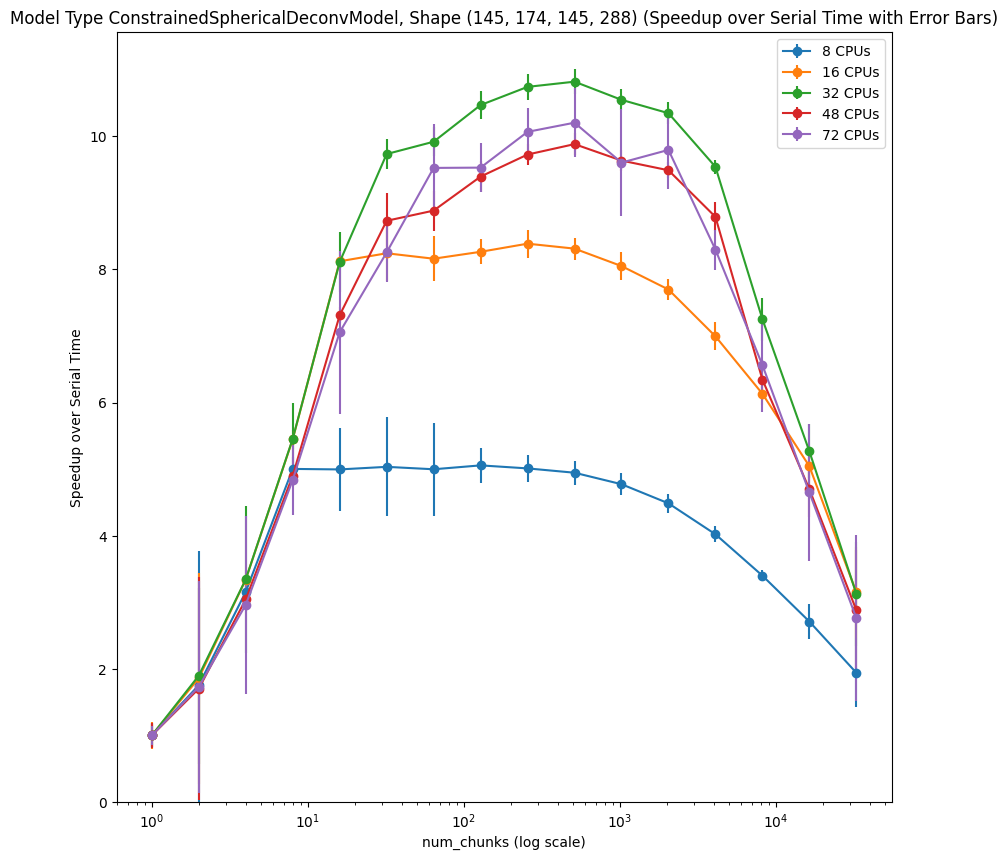
\includegraphics[width=0.8\textwidth,height=0.8\textheight]{figures/csdm_speedup.png}
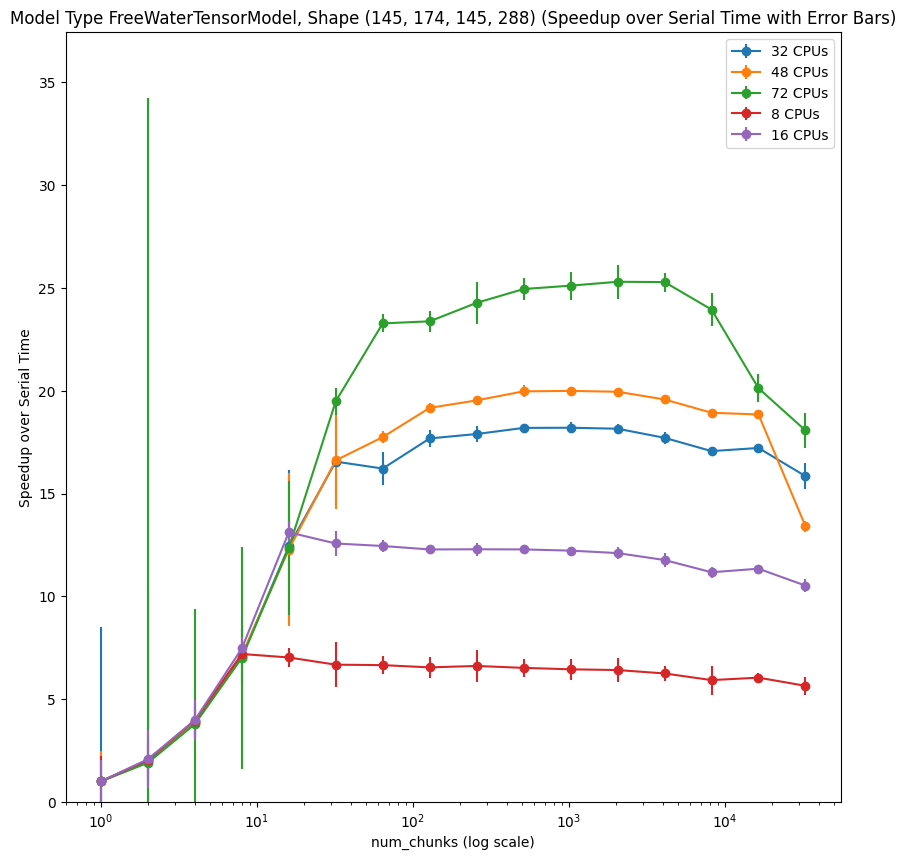
\includegraphics[width=0.8\textwidth,height=0.8\textheight]{figures/fwdtim_speedup.png}

Efficiency decreases as a function of number of CPUs, but is still
rather high in many configurations. Efficiency is also considerably
higher for the free water tensor model, which is consistent with our
expectations given that it is more computationally expensive per voxel
and therefore ray overhead would have less effect. The high efficiency
of 8 core machines suggests that the most cost-effective configuration
for processing may be relatively cheap low core machines.

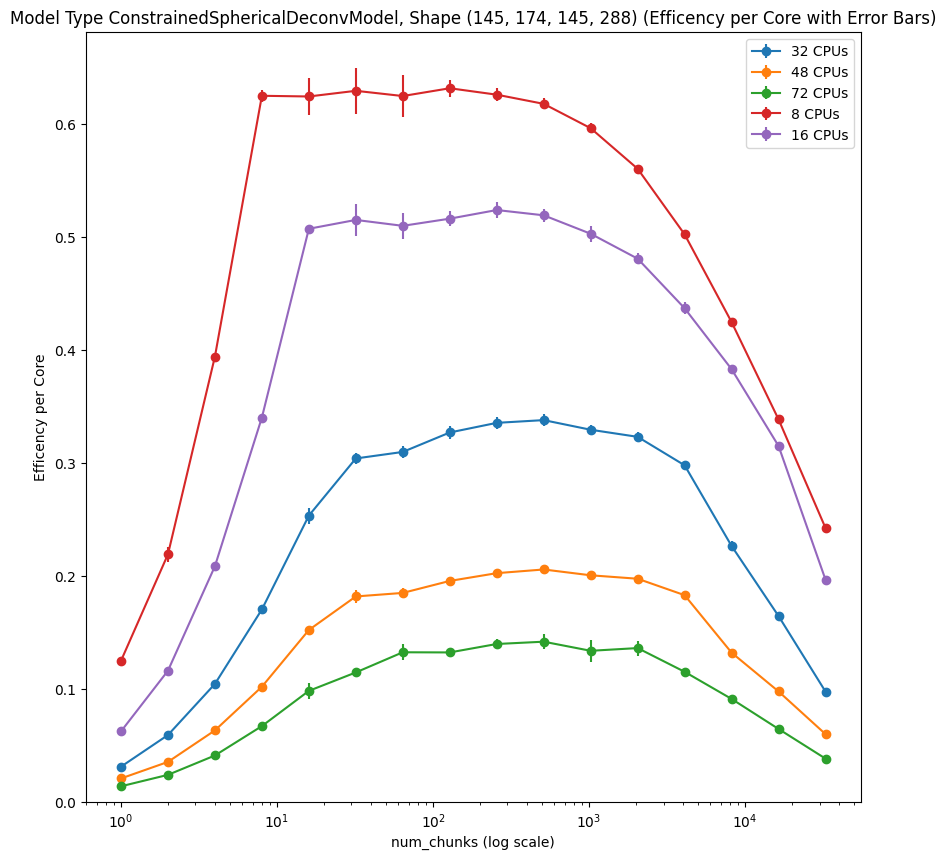
\includegraphics[width=0.8\textwidth,height=0.8\textheight]{figures/csdm_efficency.png}
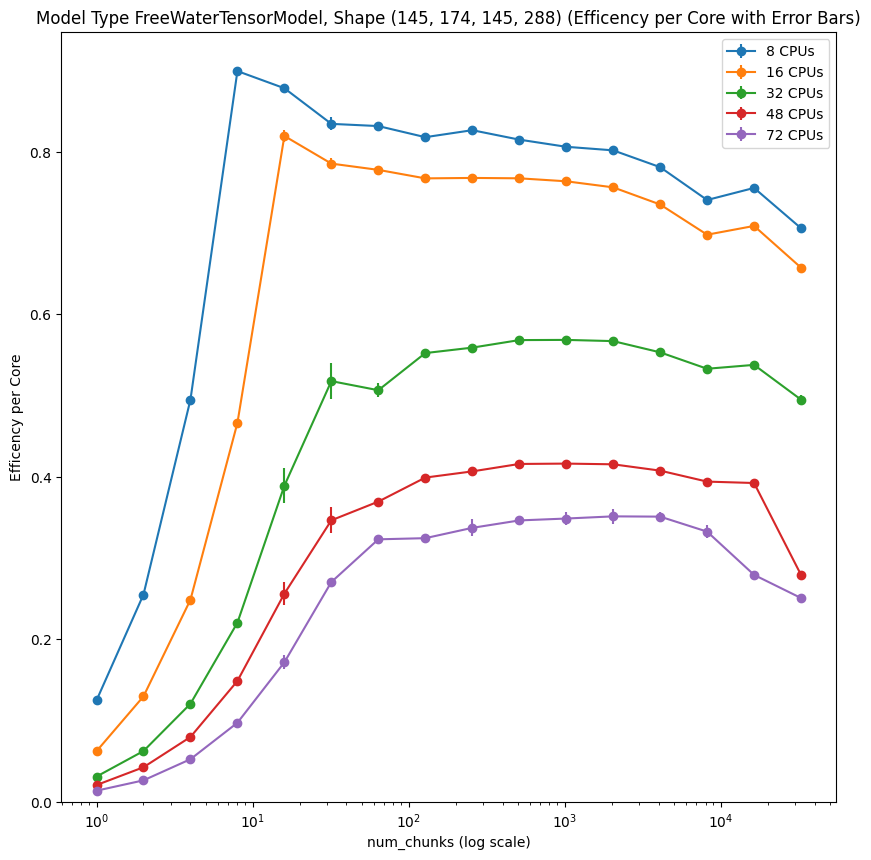
\includegraphics[width=0.8\textwidth,height=0.8\textheight]{figures/fwdtim_efficency.png}

We can also look at peak efficiency per core (efficiency at the optimal
number of chunks for the given parameters), relative to the number of
cores for both models. What's interesting is that we see a very similar
relationship between both models, with the fwdti model being higher by
almost the same amount for all core counts. This suggests that models
such as fwdti that are more computationally expensive per voxel will see
better speedups due to the overhead of parallelization being lower
relative to the total cost. Interestingly increasing core counts doesn't
further increase the benefit of parallelization relative to overhead,
which suggests that ray overhead may be very linearly related to the
number of cores.

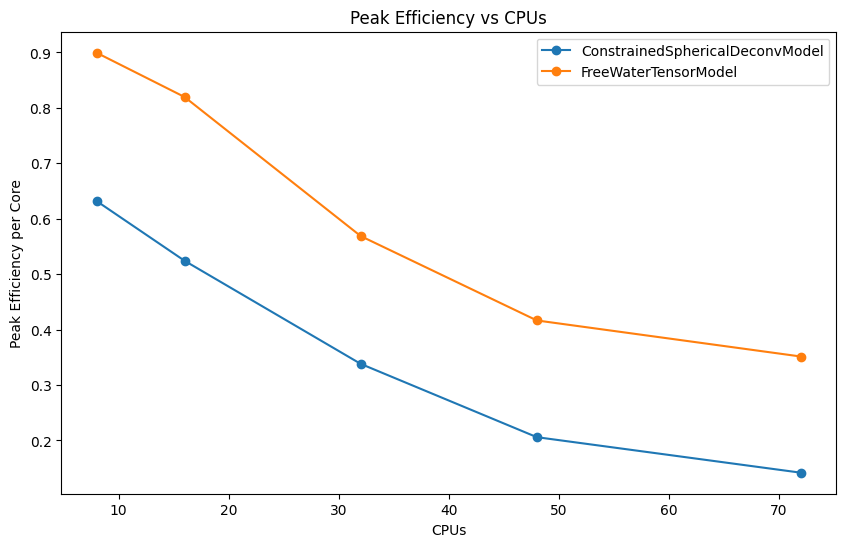
\includegraphics{figures/efficency_vs_cpus.png}

Ray tends to spill a large amount of data to the disk and does not clean
up afterward. This can quickly become problematic when running multiple
consecutive models. Within just an hour or two of running, Ray could
easily spill over 500gb to disk. We have implemented a quick fix for
this within our model as follows:

\begin{Shaded}
\begin{Highlighting}[]
    \ControlFlowTok{if}\NormalTok{ engine }\OperatorTok{==} \StringTok{"ray"}\NormalTok{:}
        \ControlFlowTok{if} \KeywordTok{not}\NormalTok{ has\_ray:}
            \ControlFlowTok{raise}\NormalTok{ ray()}

        \ControlFlowTok{if}\NormalTok{ clean\_spill:}
\NormalTok{            tmp\_dir }\OperatorTok{=}\NormalTok{ tempfile.TemporaryDirectory()}

            \ControlFlowTok{if} \KeywordTok{not}\NormalTok{ ray.is\_initialized():}
\NormalTok{                ray.init(\_system\_config}\OperatorTok{=}\NormalTok{\{}
                    \StringTok{"object\_spilling\_config"}\NormalTok{: json.dumps(}
\NormalTok{                        \{}\StringTok{"type"}\NormalTok{: }\StringTok{"filesystem"}\NormalTok{, }\StringTok{"params"}\NormalTok{: \{}\StringTok{"directory\_path"}\NormalTok{:}
\NormalTok{                         tmp\_dir.name\}\},}
\NormalTok{                    )}
\NormalTok{                \},)}

\NormalTok{        func }\OperatorTok{=}\NormalTok{ ray.remote(func)}
\NormalTok{        results }\OperatorTok{=}\NormalTok{ ray.get([func.remote(ii, }\OperatorTok{*}\NormalTok{func\_args, }\OperatorTok{**}\NormalTok{func\_kwargs)}
                          \ControlFlowTok{for}\NormalTok{ ii }\KeywordTok{in}\NormalTok{ in\_list])}

        \ControlFlowTok{if}\NormalTok{ clean\_spill:}
\NormalTok{            shutil.rmtree(tmp\_dir.name)}
\end{Highlighting}
\end{Shaded}

There seems to be an inverse relationship between the computational cost
per voxel and the speedup that you get from parallelization. This is why
CSD speedup is maximal for 32 cores.

We have also made a rough approximation of the total cost of computation
relative to the number of CPUs. Because all tests were run on a
`'c5.18xlarge'' machine, and the docker container was simply limited in
its access to cores, This approximation makes the following assumptions
to estimate the cost of using smaller machines: It assumes that the only
differentiating factor between aws c5 machines' performance is the
number of CPUs, which may not be true for several reasons, such as total
memory available, memory bandwidth, and single-core performance. With
this approximation, we see that cost increases as a function of CPUs.
This suggests that using the smallest machine that still computes in a
reasonable amount of time is likely the best option.

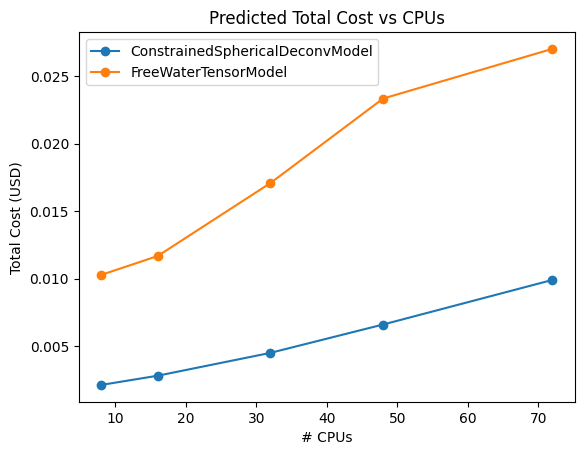
\includegraphics[width=0.8\textwidth,height=0.8\textheight]{figures/cost_vs_cpus.png}

\section{Discussion}\label{discussion}

\subsection{Acknowledgments}\label{acknowledgments}

This work was funded through NIH grant EB027585 (PI: Eleftherios
Garyfallidis) and a grant from the Chan Zuckerberg Initiative Essential
Open Source Software program (PI: Serge Koudoro).



\end{document}
